\section{Standard SIR model with logistic grow}
We use the standard population model with logistic grow reported
\cite{Schaefer2009}, see table for parameter description. To introduce the 
vaccination and treatment as mitigation control policies, we firs deal with the
uncontrolled dynamics described by:
\begin{equation}\label{eqn:SIR}
	\begin{aligned}
		\frac{dS}{dt} &=
			\mu N  
			- \beta \frac{S I}{N} 
			- \mu \frac{N}{K} S ,
		\\
		\frac{dI}{dt} &=
			\beta \frac{S I}{N}
			- (\gamma + \delta) I
			- \mu \frac{N}{K} I,
		\\
		\frac{dR}{dt} &= 
			\gamma I 
			- \mu \frac{N}{K} R ,
		\\
		S(0) &= S_0, \quad
		I(0) = I_0, \quad
		R(0) = R_0,
		\\
		N &= S + I +R,
		\\
		\frac{dN}{dt} &=
			\mu N 
			\left(
				1 - \frac{N}{K}
			\right).
	\end{aligned}
\end{equation}

Given initial population sizes $S_0, I_0, R_0$, the goal is to determine the best policy to
mitigate the outbreak described by the SIR model \eqref{eqn:SIR} and optimize a regarding  cost. In this context, the policies are Lebesgue measurable bounded functions
which optimize a given convex functional cost. For example, \citeauthor{Schaefer2009} pursue to minimize the infected population described by \eqref{eqn:SIR} while minimizing the cost of vaccination $u_1$ and treatment $u_2$. In symbols, the authors seek to minimize the objective functional
\begin{equation}
	\label{eqn:sir_logistic}
  \begin{aligned}
      & \int_{0}^T	
    		\left[
    			B_1 I(t) 
    			+ B_2 \left[\frac{R(t)}{K}\right]^m [u_1(t)]^2 + B_3 [u_2(t)]^2
    		\right] dt,
    		\qquad  m\geq 1,
      \\
    \text{subject to}
  \\
    \frac{dS}{dt} &=
			\mu N  
			- \beta \frac{S I}{N} 
			- \mu \frac{N}{K} S - u_1(t) S,
		\\
		\frac{dI}{dt} &=
			\beta \frac{S I}{N}
			- (\gamma  + \mu + \delta) I 
			- \mu \frac{N}{K} I
			- u_2(t) I,
		\\
		\frac{dR}{dt} &= 
			\gamma I 
			- \mu \frac{N}{K} R 
			+ u_1(t) S 
			+ u_2(t) I,
		\\
		S(0) &= S_0, \quad
		I(0) = I_0, \quad
		R(0) = R_0. \quad
	\end{aligned}
\end{equation}
%
%
Here $S$, $I$, $R$ respectively denotes the epidemiological
compartments for susceptible, infected and recover classes. Note 
that entire population $N=S+I+R$ obeys the logistic growth described by the
last equation of model \eqref{eqn:SIR}. \Cref{tbl:sir_logistic} encase a 
description and the values used to obtain \Cref{fig:figure1sirlog}.

\begin{table}[htb]
  \begin{center}
    \begin{tabular}{@{}rll@{}} 
      \toprule
      &
      \multicolumn{1}{c}{\textbf{Description}}
      & 
      \multicolumn{1}{c}{\textbf{Value}}
      \\
        \midrule
        $\beta$
          & Incidence rate
          & \SI{0.05}{day^{-1}}
      \\
      $\gamma$
        & Infect time
        & \SI{0.1}{day^{-1}}
      \\
      $\mu$
        & Intrinsic growth rate
        & \SI{0.00004}{day^{-1}}
      \\
        $K$
        & Carrying capacity
        & \num{5000}
      \\
      $\delta$
        & Death rate due to disease
        & \SI{0.1}{day^{-1}}
      \\
      \\  
      $B_1$,$B_2$,$B_3$
        & Weight for infected population,
        & \num{1.0}, \num{100}, \num{1000}
        \\
        & vaccination, and treatment 
      \\
      $u_1^{\max}, u_2^{\max}$
        & Max vaccination and treatment rates
        & \SI{0.1}{day^{-1}}, \SI{0.6}{day^{-1}}
      \\
      \\
      && \textbf{Initial Conditions}
      \\
      \cmidrule{3-3}
      && $S_0 = \SI{4500}{humans}$
      \\
      && $I_0 = \SI{499}{humans}$
      \\
      && $R_0 = \SI{1}{human}$
      \\
      \bottomrule
    \end{tabular}
    \caption{Parameter description and simulation values for the optimal problem
      \eqref{eqn:sir_logistic}
    }
    \label{tbl:sir_logistic}
	\end{center}
\end{table}
%
\begin{figure}
  \centering
  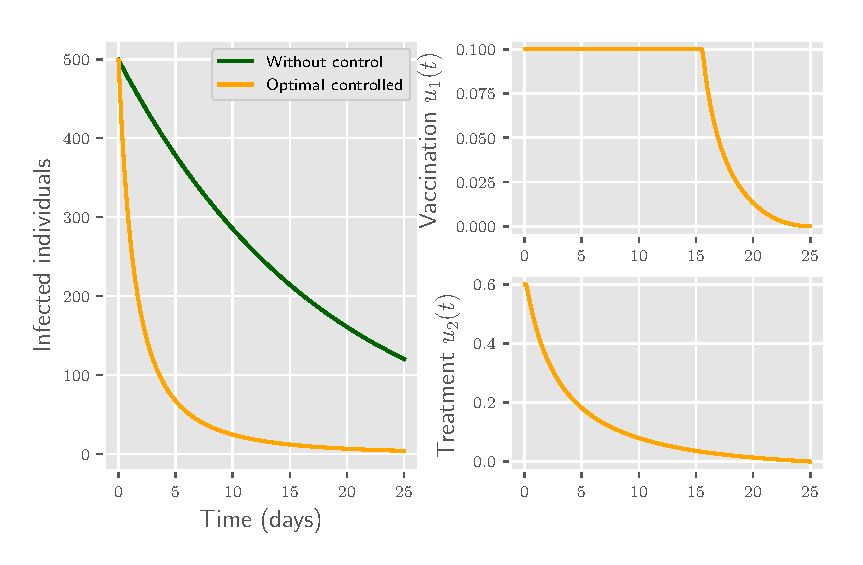
\includegraphics{Figures/figure_1_sir_log}
  \caption{}
  \label{fig:figure1sirlog}
\end{figure}

